\documentclass{article}
\usepackage{amsmath}
\usepackage{tikz}

\newcommand{\beff}{\ensuremath{b_{\mathrm{eff}}}}

\title{Lit. Review for Chapter 2}
\author{Nat Lund}

\begin{document}
\maketitle

After reading and summarizing a bunch of papers, I have now organized my folder of Reference Papers into the following subfolders:
\begin{itemize}
    \item Pure Slip --- Experimental
    \item Pure Slip --- Theory, including MD
    \item Mixed Slip Surfaces
    \item Mixed Slip Flow
    \item Effective Slip Lengths
\end{itemize}

The first two categories regarding Pure Slip went into Chapter 1.

This document is a literature review of the remaining three categories --- on mixed slip and effective slip, which will go into Chapter 2.

\section*{Contents}

\begin{itemize}
\item Mixed Slip Surfaces

Whole bunch of crap here, lotus leaves, Fakir effect surfaces, nanobubbles.

Onda Shibuchi Satoh Tsuji Langmuir 1996 \\
Barthlott and Neinhuis Planta 1997 \\
Neinhuis and Barthlott, Annals of Botany 1997 \\
Tyrrell and Attard, PRL 2001 \\
Tyrrell and Attard, Langmuir 2002 \\
Qu\'{e}r\'{e}, Nature Materials 2002 \\
Koishi et al PRL 2004 \\
Zhang Maeda Craig Langmuir 2006 \\
Kusumaatmaja Yeomans Langmuir 2007 \\
Yang et al Langmuir 2007 \\
Zhang Khan Ducker PRL 2007 \\
Sbragaglia et al PRL 2007 \\
Zhang Quinn Ducker Langmuir 2008 \\

\item Mixed Slip Flow

Zhu and Granick PRL 2002 \\
Cottin-Bizonne etal Nature Materials 2003 \\
Bonaccurso Butt Craig PRL 2003 \\
Lauga and Brenner PRE 2004 \\
Choi and Kim PRL 2006 \\
Vinogradova and Yakubov PRE 2006 \\
Choi et al PoF \\
Joseph et al PRL \\
Steinberger et al Nature Materials 2007 \\
Kunert and Harting PRL 2007 \\
Hyv\"{a}luoma and Harting PRL 2008 \\
Kunert Harting and Vinogradova PRL 2010 \\
Lee and Kim Langmuir 2011 \\

\item Effective Slip Length

Philip ZAMP 1972 \\
Einzel, Panzer and Liu PRL 1990 \\
Lauga and Stone JFM 2003 \\
Tretheway and Meinhart  PoF 2004 \\
Cottin-Bizonne etal EurPhysJE 2004 \\
Sbragaglia and Prosperetti PoF 2007 \\
Ybert etal PoF 2007 \\
Hendy and Lund PRE 2007 \\
Ng and Wang PoF 2009 \\
Davis and Lauga PoF 2009a \\
Davis and Lauga PoF 2009b \\
Ng and Wang Microfluid nanofluid 2010 \\
Davis and Lauga JFM 2010 \\

\end{itemize}

\section*{Mixed Slip Surfaces}

\subsubsection*{Onda et al Langmuir 1996}
``Super-Water-Repellent Fractal Surfaces"

Discuss the theoretical contact angle of a rough surface.  Make a `super-water-repellent fractal surface' made of alkylketene dimer.  It has a contact angle of 174$^{\circ}$.

\subsubsection*{Barthlott and Neinhuis, Planta 1997}
They note that water repellency in plants is mainly caused by wax crystalloids which cover the surface `in a regular microrelief of about 1 -- 5 $\mu$m in height.
Back in 1993 they were doing SEM micrographs of the leaf surfaces of some 10,000 plant species.  They noticed that \emph{flat} surfaces always had to be cleaned before examination, while those with surface wax crystals were almost completely free of contamination.  They study this systematically.  The lotus leaf has very pronounced self-cleaning properties  --- making it a symbol of purity in Asian religions, so they dub it the `lotus effect'.

They have a partially-convincing explanation:  dust particles tend to be hydrophilic.  Also they sit on top of the roughness peaks, so that total surface contact area is low.  Thus, when a nearly-spherical water droplet hits the dust particle, the attraction between particle and water droplet is greater than the attraction between particle and surface. So the dust particle is eaten by the droplet, which rolls rapidly off the leaf.


\subsubsection*{Neinhuis and Barthlott, Annals of Botany 1997}

SEM studies of 200 water-repellent plant species.  They find that the most water-repellent leaf surfaces have `convex' microstructures in a thick layer of wax.


\subsubsection*{Tyrrell and Attard, PRL 2001}

Abstract: "Imaging of hydrophobic surfaces in water with tapping mode atomic force microscopy reveals them to be covered with soft domains, apparently nanobubbles, that are close packed and irregular in cross section, have a radius of curvature of the order of 100 nm, and a height above the substrate of 20 -- 30 nm."

\subsubsection*{Tyrrell and Attard, Langmuir 2002}
More AFM images of what they believe to be nanobubbles. The propose them to be the source of the `hydrophobic force' -- a force that suddenly pulls two hydrophobic surfaces together when they get close enough.

\subsubsection*{Qu\'{e}r\'{e}, Surface Chemistry 2002}
A readable, high-level description of Fakir droplets. The money quote is the last few sentences of the paper:

``On a superhydrophobic solid, however, drops seem to move over a dynamic film of air --- which makes the friction comparable to that experienced by a raindrop falling in air.  But what happens if these textured solids are fully immersed in a pool of water?  Will the water still slide on them?  Except for a few controversial studies, this question still remains open, and designers of boats and swimsuits impatiently await an answer."


\subsubsection*{Koishi et al, PRL 2004}
Not important.  MD simulation nanoparticles in water, at close proximity.  When the nanoparticles were instantly switched to hydrophobic, a nanobubble nucleated between them.


\subsubsection*{Zhang, Maeda and Craig, Langmuir 2006}
Studies on the properties of nanobubbles.  They are able to induce nanobubbles, giving them reliablity.  They are similar to macro-scale bubbles, except for having a much larger contact angle, and thus larger radius of curvature.  Once formed, they hang around for hours.  ``... this apparent still remains a well-recognized mystery."

\subsubsection*{Kusumaatmaja and Yeomans, Langmuir 2007}
They investigate the hysteresis in contact angle on superhydrophobic surfaces.


\subsubsection*{Yang et al. Langmuir 2007}
Lots of experimental arcana on inducing nanobubbles, in terms of the effect of temperature, dissolved gases etc. etc.

\subsubsection*{Zhang, Khan and Ducker, PRL 2007}
Experimental proof that a very thin (5 -- 80 nm) gas phase can exist for a long time (more than an hour) on a hydrophobic surface immersed in water.  They use infrared spectroscopy to prove its there.  The gas phase is of course nanobubbles.  They show that the average pressure is approximately atmospheric, explaining the relatively long lifetime.

\subsubsection*{Sbragaglia et al, PRL 2007}
Not important.  ``Spontaneous breakdown of Superhydrophobicity"

\subsubsection*{Zhang, Quinn and Ducker, Langmuir 2008}
The big nanobubble paper that we got a draft of.

More experimental evidence for gaseous nanobubbles at the surface.  They are able to routinely prepare hydrophobic surfaces with or without nanobubbles.  The solvent excahnge method they use is also a common cleaning technique; therefore, nanobubbles may inadvertently be formed in various slip experiments.  Nanobubbles form much more easily on rough surfaces; sometimes even without the solvent exchange technique.
The gas pressure in them is 1.0 -- 1.7 atmospheres, consistent with the Laplace pressure calculated from their radius of curvature.  The air bubbles are stable for at least days, while CO2 bubbles only last a few hours.


\section*{Mixed Slip Flow}

\subsubsection*{Zhu and Granick PRL 2002}
Experiment using a modified SFA with 5 different surfaces, from molecularly smooth to roughness of 6 nm. Slip length inferred from viscous drainage force as function of distance $D$. $D=0$ was set at adhesive contact in air. Thus, the $D=0$ level could be well below the tops of the peaks. No effort was made to account for this.

Results: For molecularly smooth surface, a flow dependent slip length of up to 35 nm. Roughness suppresses slip, with 6 nm of roughness giving no slip at the flow rates studied.

\subsubsection*{Cottin-Bizonne etal Nature Materials 2003}
An MD study of a Lennard-Jones fluid. The first discovery of the fact that roughness could \emph{increase} slip. At low enough pressures, partial dewetting occurs: the fluid spontaneously goes into the Cassie state. Then the fluid `sees' a surface partly made of vapour. High slip results.

They have a flat surface, giving slip lengths in the range 20-25$\sigma$. Then they add square `dots' --- they mean posts, bloody French. With the dots, slip length is reduced down to 2$\sigma$. At low pressure, the fluid enters the Cassie state, giving slip lengths up to 57$\sigma$. With very narrow posts --- 4.9$\sigma$ wide, slip lengths could reach 130$\sigma$.

The slip length was calculated with zero plane at the bottom of the cavities.


\subsubsection*{Bonaccurso Butt Craig PRL 2003}
Demonstrate that in a completely wetting system (contact angle zero), roughness \emph{increases} slip. They use an AFM with a glass sphere approaching a flat silicon wafer. Clean silicon had a roungess of 0.7 nm rms. Etching with KOH roughened it to 4.0 and 12.2 nm rms.

They discuss the importance of defining the zero distance. Sensibly they end up defining the zero at the tops of the peaks, as this is the first point of contact in an experiment.

They fit data using Vinogradova's model. The best fit is when they fix the slip length on the (almost smooth) glass sphere at about 43 nm, and then the slip length on the substrate increases with roughness. They increase the viscosity and approach velocity separately to increase the effect. Data:

\begin{tabular}{l l l l}

Roughness rms (nm) & Normal & High $\mu$ & High $v$ \\
0.7                & 0      & 0          & 0        \\
4.0                & 1      & 20         & 135      \\
12.2               & 3.5    & 225        & 900      \\

\end{tabular}

As you can see, with normal viscosity but high approach velocity, a slip length of almost a micron is seen!

These guys understand that putting the zero in the wrong place totally affects the apparent slip lengths, but don't quite develop a full critique.

\subsubsection*{Lauga and Brenner PRE 2004}

Inspired by the large slip found in Zhu and Granick PRL 2001, these guys develop a theory to explain it: a ``leaking mattress" effect.  In the dynamic SFA test for slip, the probe repeatedly slams into a surface. Assume the surface is nearly completely covered with bubbles. Then as the probe approaches the surface, the increase in pressure causes the bubbles to shrink --- both from compression of the gas and diffusion of the gas into the liquid.  The reduced bubble size widens the channel width, making drainage easier.  Thus, the drainage force is reduced compared to what it would be at the same separation at a slower approach speed.  Hence, a shear-dependent slip effect appears.

The model parameters are area fraction coverage, bubble radius of curvature and internal contact angle of the bubble.  They fit the model to the data of Zhu and Granick PRL 2001. The model was not sensitive to radius of curvature: best fit at 10 nm, but very similar in range 1 - 50 nm.  Best fit was with contact angle $120^{\circ}$, only slightly more than the macroscopic value of $110^{\circ}$. Finally, the best fit was with a surface coverage of 99\%! 

\subsubsection*{Choi and Kim PRL 2006}

These guys made a `nanoengineered superhydrophobic surface'. Probably the first to deliberately make a surface for maximum slip.  They made `nanoturf', silicon nanoposts about 1 -- 2 $\mu$m high, spaced about 0.5 -- 1 $\mu$m apart, rendered hydrophobic by a 10 - 20 nm thick coating of Teflon.  They estimate the air fraction of the surface to be ~ 60\%.

A commercial cone-and-plate rheometer was used to measure slip length.  They find a humungous ~20 $\mu$m slip length for water, and 2.5 times greater 50 $\mu$m slip length for a 30\% glycerine solution.  They expect this, since the viscosity of the glycerine solution is 2.5 times higher.

In a personal communication, C\'{e}cile Cottin-Bizonne suspects this result is bollocks.


\subsubsection*{Vinogradova and Yakubov PRE 2006}

These guys finally figure out that the position of the nominal surface is critical.
They used a purpose built AFM device in which a roughened sphere was tapped onto a smooth plane.  The sphere had an r.m.s. roughness of 10 - 11 nm, and a maximum peak-to-valley distance of 45 nm. The plane had an r.m.s. roughness of 0.5-0.8 nm and maximum peak-to-valley distance of less than 2.5 nm.

With separation distance taken from peak of sphere to peak of surface, a reduction in drainage force was observed, compared to the case of a smooth sphere tapping a smooth plane.  But the reduction was not due to slip.  The force was equivalent to that of a smooth sphere whose surface was located at an intermediate position between peaks and valleys of the roughness.

Thus they reveal that the position of the boundary is critical: if the boundary is taken to be at the valleys of roughness, then roughness reduces slip.  Conversely, if the boundary is taken to be at the tops of the peaks, then roughness increases slip.  In both cases, no true slip need exist --- only the effective boundary position changes. 
They note:

``We believe our paper entirely clarifies the situation with flow past rough surfaces, highlights reasons for existing controversies, and resolves apparent paradoxes."

\subsubsection*{Choi et al PoF 2006}

Last sentence of their abstract: ``This paper is the first to use \emph{nanoscale} grating patterns and to measure their effect on liquid flows in microchannels."

They fabricate a `well-defined nanograte' with a pitch of ~230 nm: ridges ~500 nm high and ~50 nm wide separated by a gap of ~180 nm.  The nanograting was fabricated on the walls of microchannels, with the ridges aligned either parallel to the direction of flow, or transverse to it, and either left hydrophilic, or rendered hydrophobic with Teflon. Flow experiments were carried on microchannels of heights ~3, ~5 and ~11 $\mu$m.

The slip length data showed a lot of scatter.  For parallel flow, there was a clear distinction between hydrophilic and hydrophobic surfaces: $30\pm16$ nm slip length for hydrophilic, and $143\pm35$ nm for hydrophobic.

For transverse flow, the distinction is not as clear: insignificant slip, $0 \pm 17$ nm for hydophilic, and $61\pm44$ nm for hydrophobic.

They can only measure slip length to a resolution of ~30 nm, so cannot assume any slip on the solid ridges.  They believe that there is \emph{air} in the grate troughs of the hydrophobic surface, while \emph{water} wets and fills the grate troughs of the hydrophilic surface.

Noting that the air fraction is ~0.7, they use the effective slip length expressions of Lauga and Stone 2003, and Cottin-Bizonne et al 2004, using infinite slip over air, and slips of 0, 30, 60  and 90 nm on the solid ridge top.  They find that air fraction 0.7 and slip of 30 nm on the solid predicts an effective slip length of 100 nm --- comparing well with experimental mean 143 nm and standard deviation of 35 nm.


\subsubsection*{Joseph et al PRL 2006}

(Where the Lyon crew suspect Choi and Kim's $20\mu$m slip is bollocks.)
The Lyon microfluidic research group fabricate forests of carbon nanotubes, of diameter 50 - 100 nm, spaced 100-250 nm apart, which coat the walls of microchannels. If they functionalize them in the gas phase to make them hydrophobic, the CNTs remain unchanged.  But if they functionalize them in the liquid phase (ethanol), the nanotubes clump together like wet hair.  By controlling the liquid evaporation rate they can make surfaces with inter-clump length scales $L$ of 1.7, 3.5,and 6 $\mu$m.

They then do particle image velocimetry to get flow profiles, getting slip lengths.
In the Cassie state, the surfaces with length scales 1.7, 3.5 and 6 $\mu$ give effective slip lengths of roughly 0.4, 1.0 and 1.4 $\mu$m, respectively.

They fit this data with their theoretical expression from Cottin-Bizonne 2004.  Noting that this regime is not exactly covered by their theory, they assume perfect slip over gas, and find that the expression reduces to $b_{\mathrm{eff}} = \alpha(\phi_{\mathrm{solid}}) L$.  In other words, in this regime, slip length depends linearly on length scale $L$, with only weak dependence on area fraction of solid $\phi_{\mathrm{solid}}$.  The results fit best to this expression with an area fraction $\phi_{\mathrm{solid}}$ of 0.15 -0.20.  This is `remarkably consistent' with the experimentally estimated $\phi_{\mathrm{solid}}$ of 0.10.

Finally, they point out that their results are an order of magnitude smaller than the ~20$\mu$m slip length reported for a superhydrophobic nanoforest by Choi and Kim.  They point out that rheological methods lack the sensitivity to measure surface effects, and moreover that neglecting the post structure `fails to interpret slippage on nanopatterned surfaces'.


\subsubsection*{Steinberger et al Nature Materials 2007}

They build a flat surface, covered with holes 1.3 $\mu$m wide and 3.5 $\mu$m deep.  They do SFA tests of slip length on this surface.

In the Wenzel state, with water in the holes, they find an effective slip length of $105 \pm 10$ nm --- that is, the effective no-slip plane lies 105 nm below the \emph{top} of the holes.

In the Cassie state, with air trapped in the holes, they find a \emph{lower} slip length: an effective no-slip plane only $20\pm 10$ nm below the flat surface.  This puzzles them, so they eventually estimate that the microbubbles protrude 200 - 400 nm above the surface, with the meniscus subtending an angle of $30^{\circ} < \theta < 60^{\circ}$. Is this protruding meniscus the cause of the low slip lengths?

They test this numerically, with FEM (Comsol). They find that a flat bubble ($\theta=0^{\circ}$) gives maximum slip length --- about 160 nm.  Any increase in $\theta$ decreases slip, with $\theta > 45^{\circ}$ giving less slip than the Wenzel state.  The numerics are in quantitative agreement with their experimentally estimated $30^{\circ} < \theta < 60^{\circ}$.

Once again, this demonstrates the importance of defining \emph{where} your nominal surface is.



\subsubsection*{Kunert and Harting PRL 2007}

These guys have read and agreed with Vinogradova and Yakubov's 2006 paper pointing out the importance of deciding where your nominal surface is.  They use V and Y's concept of an `effective no-slip plane', typically located between the peaks and valleys of the surface roughness.

They do a bunch of numerical simulations using lattice Boltzmann methods, on 4 different surfaces.  Each surface has a minumum and maximmum height, $h_{\mathrm{min}}$ and $h_{\mathrm{max}}$, and an \emph{average} height $R_{a}$.  They calculate the position of the effective no-slip plane.  For `symmetric' surfaces like sine waves, triangle waves and square waves, $R_{a} = h_{\mathrm{max}}/2$. For sine wave surfaces, making the sine wave steeper (reducing the period) raised the height of $h_{\mathrm{eff}}$.  In all cases $h_{\mathrm{eff}}$ was at least 1.69 times $R_{a}$.

They note that $h_{\mathrm{eff}}$ is always greater than $R_{a}$.  If the surface has a few very tall but sparsely distributed spikes, then $R_{a}$ can be much smaller than $h_{\mathrm{max}}$, and $h_{\mathrm{eff}}$ is somewhere between them, and cannot be well approximated by either.


\subsubsection*{Hyv\"{a}luoma and Harting PRL 2008}

These guys have read Steinberger's bubble mattress paper showing that bubbles can \emph{decrease} slip because they protrude into the channel, impeding flow.  They investigate this further with lattice Boltzmann methods.  The improvement in using Lattice Boltzmann methods (rather than Steinberger's FEM) is that the bubble surface is allowed to deform under stress.

They essentially replicate Steinberger's findings: a maximum slip of about 150 nm at zero protrusion angle, plummeting down past zero slip for protrusion angle greater than about $70^{\circ}$.

Since they simulate Couette flow, they are able to investigate the shear dependence.  Higher shear deforms the bubbles, and they see a \emph{decrease} in slip length with increasing shear. This contradicts other experiments showing the onset of slip above a critical shear rate, for example.  However, they emphasize that their experiments are static (Couette flow) rather than dynamic.  In their case, shear reduces the average height of bubbles.  They think this is consistent with Kunert and Harting above, which they claim shows reduced slip from reduced roughness.  But.... these guys measure slip at the `top of the structured surface', whereas Kunert and Harting place an effective no-slip plane some distance $b$ below the tops of the roughness. So in K and H 2007, reduced roughness height gives reduced $b$.  It shouldn't do here.  I reckon its caused by the fact a deformed bubble gives steeper roughness, causing stagnancy in the lee side, thus lower surface velocity, thus lower $b$.


\subsubsection*{Kunert Harting and Vinogradova PRL 2010}

Lattice Boltzmann simulations of high-speed drainage of liquid between a smooth sphere and randomly rough plane.  A sphere of radius $R$ approaches the plane, with distance $h$ to the \emph{tops} of the roughness.

To begin with, the exact solution for a sphere approaching a smooth plane, valid for arbitrary separation is given by Brenner and Maude.  The leading term can be evaluated as:

\[ F \sim 1 + \frac{9}{8} \frac{R}{h} \]

Obviously, drag force goes to infinity as separation closes.  So sphere never touches.

Another model is that the surface has a single slip length. Then asymptotically,

\[ F \rightarrow \frac{9R}{32h} \;\;\; \mathrm{as}\;h \rightarrow 0 \]

Yet another model is that the appropriate no-slip boundary is located a distance $s$ below the top of the roughness. Then:

\[ F \sim 1 + \frac{9}{8} \frac{R}{h + s} \]

\[ F \rightarrow \frac{9R}{8s}\;\;\; \mathrm{as} \; h \rightarrow 0 \]


The last model allows the sphere to touch the plane.  The slip model does not.

They find: At distant separations, the models agree with each other.  But at close separations, there is a lower force than predicted by the conventional equation \emph{and} by the slip equation.  However, the effective no-slip plane model fits the data very well.

In conclusion, modeling a rough surface with a uniform slip plane on the top of the roughness is not as good as modeling it as a smooth no-slip plane located below the peaks of the roughness.


\subsubsection*{Lee and Kim Langmuir 2011}

These guys build a hierarchical superhydrophobic surface: nanoposts on top of microposts. They hope to get mega slip out of it.  It works up to point.  Below about 10\% area fraction of microposts, the advantage begins to disappear, and at about 4\% area fraction of microposts, the hierarchical structure gives \emph{lower} slip than the unadorned microposts.

They note that if regular microposts are rounded at the top, rather than `sharp', slip is reduced because the liquid meniscus must sag lower to get the same surface tension support.  They think that the forest of nanoposts on top of the micropost has the same effect --- the sharp right-angle edge of the micropost is blurred, so the liquid intrudes into the air gap.  Note that this happens without the liquid penetrating into the nanoposts.




\section*{Effective Slip Lengths}

\subsubsection*{John R. Philip ZAMP 1972}

\textbf{No-slip / Perfect slip \\ Flat surface \\ Parallel strips \\ Navier-Stokes flow }

The one that started it all.  John Philip uses the term no-shear to describe a surface with infinite slip.  He studies amongst other things ``Shear Flow over a Plate with a Regulary Array of Longitudinal No-Shear Slots".  The no-shear slots are parallel to the flow direction.  He generalizes the device of Karush and Young, a conformal mapping in the complex plane.

The simple Couette flow solution is:
\[ w_{1} = \tau_{\infty} y / \mu  \]
For slots of width $2a$ with centres space distance $2b$ apart:
\[ w_{3} = w_{1} + a \tau_{\infty} W_{3} / \mu \]

In the limit of $y \rightarrow \infty$:
\[ W_{3} = \alpha^{-1} \ln \sec \alpha \;\;\; \mathrm{where}\;\;\;
\alpha = \frac{\pi}{2} \frac{a}{b} \]

Thus, at infinite height:
\[ w_{1} = \frac{\tau_{\infty}}{\mu} \left(y + a W_{3}  \right) \]
that is, velocity depends linearly on height, with a simple offset, the \emph{slip length:}

\[ b_{\mathrm{eff}} = a W_{3} = a \frac{2}{\pi} \frac{b}{a} \ln \sec \frac{\pi}{2} \frac{a}{b} \]

\[ b_{\mathrm{eff}} = \frac{2b}{\pi} \ln \sec \frac{\pi}{2} \frac{a}{b} \]

In our language, the centre to centre distance $2b$ is the period of the pattern $L$.  Then $2a$ is the width of the perfect-slip slots, so that $a/b = \phi_{\mathrm{slip}}$ is the fraction of the surface that is perfect slip

Thus:
\[ b_{\mathrm{eff}} = \frac{L}{\pi} \ln \sec \frac{\pi}{2} \phi_{\mathrm{slip}} \]


\textbf{Transverse Strips\\ No-slip/Perfect-slip \\ Stokes flow \\}

J. Philip also studied flow over \emph{transverse} no-shear slots.  He was only able to use Stokes flow, not Navier-Stokes flow.  He uses the Stokes stream function.

The Couette flow solution is:
\[ \psi_{1} = \frac{1}{2} \tau_{\infty} y^{2}/\mu \]

The solution for `Shear Stokes Flow over a Plate with a Regular Array of Transverse No-Shear Slots' will be of the form:
\[ \psi_{3} = \psi_{1} + a \tau_{\infty} \Psi_{3} /\mu\]

The solution of $\Psi_{3}$ is: \[ \Psi_{3} = \frac{1}{2} Y W_{3} \]
So: 
\[ \psi_{3} = \frac{1}{2} \tau_{\infty} y^{2}/\mu
            + a \tau_{\infty} \frac{1}{2} Y W_{3} /\mu  \]            

Now, $Y$ is the nondimensionalized $y/a$. So:
\[ \psi_{3} = \frac{\tau_{\infty}}{\mu} \left( \frac{1}{2} y^{2}
            + \frac{1}{2} y W_{3} \right)  \]      

It is \textbf{very tempting} to say that $x$-velocity $u$ is given by
\[ u = \frac{\partial \psi}{\partial y} \]
Hence:
\[ u = \frac{\tau_{\infty}}{\mu} \left( y
            + \frac{1}{2} W_{3} \right)  \]
So that the slip length is:
\[ b_{\mathrm{eff}} = \frac{1}{2} W_{3}\]
which in the limit $y \rightarrow \infty$ is 
\[ b_{\mathrm{eff}} = \frac{1}{\pi} \frac{b}{a} \ln \sec \frac{\pi}{2} \frac{a}{b} \]

But \textbf{unfortunately}, $W_{3}$ is a function of $y$, so must be differentiated \emph{before} taking the limit.

So in reality:
\[ u = \frac{\tau_{\infty}}{\mu} \left( y
            + \frac{1}{2} W_{3}
            + \frac{1}{2} y \frac{\partial W_{3}}{\partial y} \right) \]
            
This is explored in another file... `JohnPhilip.tex'

At this stage, I don't know if it is possible to extract a velocity out of the stream function for transverse slots --- apparently nobody has. But in any case, Sbragaglia and Prosperetti managed to get an answer in 2003.


\subsubsection*{Einzel Panzer Liu PRL 1990}

``Boundary Condition for Fluid Flow: Curved or Rough Surfaces"

\textbf{Single Slip Length}\\
\textbf{Rough Surface}\\
\textbf{Navier Stokes flow}\\

These guys make three claims.
First, they consider the Navier slip condition:
\begin{equation} v_{\mathrm{tang}} = b \partial_{\mathrm{n}} v_{\mathrm{tang}} \end{equation}
and claim to prove that it ``represents the most general hydrodynamic boundary condition compatible with conservation laws and irreversible thermodynamics.  Its form remains valid even if the surface is curved."

Second, they also claim that the slip length $b$ has two contributions:
\begin{equation} \frac{1}{b} = \frac{1}{b_{0}} + \frac{1}{R} \end{equation}
where $b_{0}$ is the intrinsic slip length ``determined by the fraction of diffuse scattering off a flat boundary". $R$ is the radius of curvature of the boundary.

Third, they consider ``mesoscopic curvature radii, more commonly referred to as surface roughness."  They note that typical slip experiments on \emph{macroscopically} flat surfaces provide a slip length. ``The usual prejudice in interpreting these experiments is that this slip length is $b_{0}$, calculated \emph{microscopically} assuming a flat surface." But ``the measured ``effective" slip length $b_{\mathrm{eff}}$ contains the information of the appropriately averaged $b$ of Eq. (2), which depends especially on the curvature radii of the surface roughness."

They go on to prove that
\begin{equation}
b_{0} (\nabla_{k} v_{i} + \nabla_{i} v_{k}) t_{i} n_{k} = v_{i} t_{i}
\end{equation}
is equivalent to the first two equations. ``[The first] two are the physically transparent version, while Eq. (3) is frequently the computationally convenient one."

They solve these equations for rough bondaries, getting an effective slip length in terms of the intrinsic slip length.
For a `weakly varying surface' of the form
\[ y(x) = \Sigma_{n} [h_{n}^{cos} \cos (nkx) + h_{n}^{sin} \sin (nkx)] \]

they get, to order $\kappa^{2}$
\[ b_{\mathrm{eff}} = \frac{b_{0} (1-\frac{5}{4} \Sigma_{n} \kappa_{n}^{2})
 - \Sigma_{n} \kappa_{n}^{2}/nk (1 + 2nk b_{0})}
{1 + \Sigma_{n} \kappa_{n}^{2} (\frac{1}{2} +nkb_{0}) } \]
where
\[ \kappa_{n} = nk \sqrt{(h_{n}^{cos})^{2} + (h_{n}^{sin})^{2}} \]

In the ``stick" limit, $kb_{0} \ll 1$, this is
\[ b_{\mathrm{eff}} = b_{0} - \Sigma_{n} \kappa_{n}^{2} /nk \]

while in the other limit, $kb_{0} \gg 1$, this is
\[  b_{\mathrm{eff}}^{-1} = b_{0}^{-1} + \Sigma_{n} nk \kappa_{n}^{2}\]

They get a very similar result for incommensurate sine waves; so the result holds for pseudo-random roughness.

The take-home message is that even a perfect slip surface will have macroscopic stick if it is rough enough.



\subsubsection*{Lauga and Stone JFM 2003}
``Effective slip in pressure-driven Stokes flow"

\textbf{No-slip / Perfect-slip slots}\\
\textbf{Flat surface}\\
\textbf{Stokes flow}\\

Flow down a straight circular pipe. With perfect-slip slots running down the length of the pipe, (parallel), they quote John Philip's 1972 result.
 
 \[ b_{\mathrm{eff}} = \frac{L}{\pi} \ln \sec ( \frac{\pi}{2}) \phi_{slip} \]
where $\phi$ is the fraction of perfect-slip surface.  This is valid for all $\phi$ and ??$L<2\pi$ ??

When the perfect-slip strips are transverse to the flow direction, there is no analytic solution.  They derive dual series equations, one for each boundary strip, which are simultaneously true.  They solve these numerically.
With $\phi_{slip}$ fixed, the asymptotic limit of the numerical solutions as period $L \rightarrow 0$ is
\[ b_{\mathrm{eff}} = \frac{L}{2 \pi} \ln \sec ( \frac{\pi}{2}) \phi_{slip} \]
which is exactly half the solution for parallel strips.

They provide a physical interpretation of the factor of 2: An elongated body falling under its own weight falls twice as fast if it is oriented vertically than if it is oriented horizontally.



\subsection*{Tretheway and Meinhart PoF 2004 + Erratum 2006}
``A generating mechanism for apparent fluid slip in hydrophobic channels"

\textbf{Stokes flow}\\
\textbf{No-slip, Partial-slip surface}\\
\textbf{Flat surface}\\
\textbf{Naive area-weighted average of slip lengths}\\
\textbf{They don't seem to realise this}\\
\textbf{Slip length over pure gas may be sound}


The notorious (to me) `cumulative velocity' paper.
They `examine analytically flow between two infinite parallel plates, assuming nanobubbles or a depleted region form an effective air gap near the wall.'

\textbf{A. Air gap with a continuum approximation}
Assume gas layer of thickness $\delta$ and a liquid layer of thickness $2D$. Assume no shear at $y=D$ (Poiseuille type flow). The $y=0$ boundary is at the air-liquid interface (as it should be). Velocity solution:
\[ u_{continuum} = \frac{1}{2\mu_{w}} \left( \frac{dp}{dx} \right) \left[
y^{2} - 2Dy - 2 \frac{\mu_{w}}{\mu_{a}}
\left( D \delta + \frac{\delta^{2}}{2} \right)  \right] \]
% D \delta - \frac{\mu_{w}}{\mu_{a}} \delta^{2} \right] \]

Assuming Navier slip: $u(y=0) = b \frac{du}{dy}|_{y=0}$, then slip length is:
\[ b_{continuum} =  \frac{\mu_{w}}{\mu_{a}} \left( \frac{\delta^{2}}{2D} + \delta \right)  \]

Fitting this to the dodgy experiments of the time, Zhu and Granick, Pit etal suggests a gas layer height of tens of nanometers.  At this scale, the gas is not a continuum, so a rarefied gas model is used.  Then, the no-slip assumption at the air-solid interface is not valid.

\textbf{B. Air gap with rarefied gas conditions}
The Knudsen number Kn$= \lambda/\delta$, which is the ratio of mean free path $\lambda$ to length scale, is large in nanobubbles.  In these conditions, gas kinetic theory gives a slip length at the solid interface:
\[ \epsilon = \left( \frac{2 - \sigma}{\sigma} \right) \frac{2}{3} \lambda \]
where $\sigma$ is the accommodation factor, defined as 1 for diffuse reflection and 0 for specular reflection (perfect slip).

\textbf{Erratum!}

At this point we jump to the erratum published two years later.

They now realise that the gas slip length $\epsilon$ applies in the gas at the air-water interface.  There is a discontinuity in velocity going from liquid to gas --- the gas is going slower because it has partially-specular collisions with the water.
So:
\[ u_{w|y=0}-u_{g|y=0} = \left( \frac{2 - \sigma}{\sigma} \right)
 \left( \frac{2}{3} \lambda \right) \left( \frac{du_{g}}{dy} \right)
  = \epsilon \left( \frac{du_{g}}{dy} \right) \]

This gives velocity at the air-water interface of:
\[ u_{\mathrm{rare}} = \frac{1}{2\mu_{w}} \left( \frac{dp}{dx} \right)
 \left[
y^{2} - 2Dy - 2 \frac{\mu_{w}}{\mu_{a}} 
\left( D \delta + \frac{\delta^{2}}{2} + \epsilon ( 2D + \delta)  \right)
\right] \]
which is the same as the gas-stick-continuum model except for the gas slip term $\epsilon (2D + \delta)$

We'll need to know shortly that:
\[ \partial_{y} u_{\mathrm{rare}} = \frac{1}{2\mu_{w}} \left( \frac{dp}{dx} \right)
 \left[
2y - 2D
\right] \]


Now, the slip length is \emph{not} the $y$ value at which $u_{\mathrm{rare}}$ is zero.
It is the \emph{linear} extrapolation of $u_{\mathrm{rare}}$ down to zero.  The linear extrapolation is $y$ times $\partial_{y} u_{\mathrm{rare}}$ evaluated at $y=0$.

The slip length is the $y$ value solving:
\[  \partial_{y} u_{\mathrm{rare}}|_{y=0} y = u_{\mathrm{rare}}(0) \]
\[  - 2D y = - 2 \frac{\mu_{w}}{\mu_{a}} 
\left( D \delta + \frac{\delta^{2}}{2} + \epsilon ( 2D + \delta)  \right) \]
\[ y = \frac{1}{2D} 2 \frac{\mu_{w}}{\mu_{a}} 
\left( D \delta + \frac{\delta^{2}}{2} + \epsilon ( 2D + \delta)  \right)  \]
So
\[ b_{\mathrm{rare}} = \frac{1}{2D} \left( \frac{\mu_{w}}{\mu_{a}} \right)
\left( 2 D \delta + \delta^{2} + \epsilon ( 4D + 2\delta)  \right) \]

\textbf{back to original paper}

\textbf{C. Intermittent surface coverage}

Now the guts of the paper.

``Solving Stokes flow between two infinite parallel plates assuming no slip at the walls and no stress at the centerline yields the velocity equation
\[ u_{\mathrm{no-slip}} = \frac{D^{2}}{2 \mu_{w}} \left( \frac{-dp}{dx} \right)
\left[ 1 - \left( \frac{y - D}{D}  \right)^{2} \right] \]
... We combine the slip and no-slip equations in a weighted average and calculate the cumulative velocity, $u_{\mathrm{cu.}}$, by
\[ u_{\mathrm{cu.}} = \phi u_{\mathrm{slip}} + (1-\phi) u_{\mathrm{no-slip}} \]
where $\phi$ is the surface fraction covered by gas. ..., we set the cumulative velocity at the air-water interface equal to the slip length times the shear rate at the air-water interface and obtain an equation for the slip length ..."

\textbf{Back to erratum again}

\[b_{\mathrm{cu.}} = \frac{\phi}{2D} \left( \frac{\mu_{w}}{\mu_{g}} \right)
\left[ \delta^{2} + 2 \delta (\epsilon + D) + 4 \epsilon D \right]  \]

In my notation this is:
\[ b_{\mathrm{cu.}} = \phi \frac{1}{2D} \left( \frac{\mu_{w}}{\mu_{g}} \right)
\left[ 2 D \delta + \delta^{2} + \epsilon ( 4D + 2 \delta ) \right] \]
Or, 
\[ b_{\mathrm{cu.}} = \phi b_{\mathrm{rare}} \]
\emph{Duh.}

This is \%\$\#\&ing lame.  Assuming a `cumulative velocity' to be the area weighted average of slip and no-slip velocities gives a `cumulative slip length' which is the area-weighted average of slip lengths!

\textbf{Proof:}

Rewrite the no-slip velocity
\[ u_{\mathrm{no-slip}} = \frac{D^{2}}{2 \mu_{w}} \left( \frac{-dp}{dx} \right)
\left[ 1 - \left( \frac{y - D}{D}  \right)^{2} \right] \]
in a more sensible way:
\[ u_{\mathrm{no-slip}} = \frac{1}{2 \mu_{w}} \left( \frac{dp}{dx} \right)
\left[ y^{2} - 2 D y \right] \]

Then the slope is the same as that over rarefied gas:
\[ \partial_{y} u_{\mathrm{no-slip}} = \frac{1}{2 \mu_{w}} \left( \frac{dp}{dx} \right)
\left[ 2y - 2 D  \right] \]

So we have $\partial_{y} u_{\mathrm{no-slip}}=\partial_{y} u_{\mathrm{rare}}$.

I interpret their statement about calculating a slip length from the cumulative velocity as this:
\[ u_{\mathrm{cu}} = b_{\mathrm{cu}} \partial_y u_{\mathrm{cu}} \]
    \[ \phi u_{\mathrm{rare}} + (1-\phi) u_{\mathrm{no-slip}} = b_{\mathrm{cu}} \partial_y [ \phi u_{\mathrm{rare}} + (1-\phi) u_{\mathrm{no-slip}} ] \]
\[ \phi u_{\mathrm{rare}} + (1-\phi) u_{\mathrm{no-slip}} =  \phi b_{\mathrm{cu}}   \partial_y u_{\mathrm{rare}} + (1-\phi) b_{\mathrm{cu}} \partial_y u_{\mathrm{no-slip}} \]
Divide both sides by $\partial_{y} u_{\mathrm{no-slip}}=\partial_{y} u_{\mathrm{rare}}$.
\[ \phi \frac{u_{\mathrm{rare}}}{\partial_y u_{\mathrm{rare}}} + (1-\phi)\frac{ u_{\mathrm{no-slip}}}{\partial_y u_{\mathrm{no-slip}}} =  \phi b_{\mathrm{cu}}    + (1-\phi) b_{\mathrm{cu}}  \]
\[ \phi b_{\mathrm{rare}} + (1-\phi)b_{\mathrm{no-slip}} =
  \phi b_{\mathrm{cu}}    + (1-\phi) b_{\mathrm{cu}}  \]
\[b_{\mathrm{cu}} = \phi b_{\mathrm{rare}} + (1-\phi)b_{\mathrm{no-slip}} \]
which is the area-weighted average of slip lengths.

Obviously $ b_{\mathrm{no-slip}} = 0 $ so that $ b_{\mathrm{cu.}} = \phi b_{\mathrm{rare}} $

\textbf{Summary:}

In their erratum, it is obvious that $ b_{\mathrm{cu.}} = \phi b_{\mathrm{rare}} $. But they do not mention this.  

In their definition of `cumulative velocity', there is an implicit `cumulative slip length' defined as $ b_{\mathrm{cu}} = \phi b_{\mathrm{rare}} + (1-\phi)b_{\mathrm{no-slip}} $.  They do not mention this.

Their slip length over a pure gas surface comes from gas kinetic theory, and may be sound.

\vspace{1em}
They do not use a consistent form for the velocity equations in the original paper.  This may have obscured the fact that their effective slip length is a naive area-weighted average.  I have tried to use a consistent form in my summary above.

Their cumulative slip length in the original paper is more complicated; the one in the erratum is given above.  Their original one may reduce to the one above, I don't know, and at this point I am sufficiently unimpressed to not give a damn.


\textbf{Note on notation.}

To me, the slip length formula should be written so that the  biggest term comes first.  For liquid channel of width $D$, over air gap of width $\delta$,
\[ b_{\mathrm{cont.}} = \frac{\mu_{w}}{\mu_{a}} 
\left( \delta + \frac{\delta^{2}}{2D}  \right) \]

Then over rarefied gas that may slip on solid and liquid:
\[ b_{\mathrm{rare}} = \left( \frac{\mu_{w}}{\mu_{a}} \right)
\left[ \delta + \frac{\delta^{2}}{2D} + \epsilon \left( 2 + \frac{\delta}{D} \right)  \right] \]
which is of the same form. $\epsilon$ may be as small as $\frac{2}{3}\lambda$, the mean free path, but $\epsilon \rightarrow \infty$ as gas collisions become more and more specular.


\subsection*{Cottin-Bizonne etal Eur. Pys. J. E. 2004}

\textbf{Flat Surface\\Stripes:\\
 No-slip/Perfect-slip; No-slip/partial-slip;Partial-slip/perfect-slip\\ Stokes flow}

The first appearance of the harmonic mean formula.

Cecile and colleagues do a bunch of MD, in which they observe the dewetting transition, wherein the liquid sits on top of the posts, giving a large slip length.
Then they do some analytical work to predict the effective slip length.

They assume a flat surface of spatially varying intrinsic slip length.  They assume Stokes `creeping' flow. They describe the slip length function with 2D Fourier components.  They put all this into a pair of mathematical equations.  These analytically derived equations are then solved numerically via a matrix inversion.

The semi-analytic results are examined for different regimes.

\textbf{Alternating Stripes, No-slip, Perfect-slip}

They compare their numerics to the analytic results of John Philip and Stone and Lauga.  There is excellent agreement.  They feel good, and feel their technique is trustworthy.

\textbf{Alternating Stripes, No-slip, Partial-slip}

For stripes of no-slip and finite slip length $b_{\mathrm{slip}}$, with period $L$:
They find that the effective slip length is fixed by the smaller of the two lengths, $b_{\mathrm{slip}}$ and $L$.

$\bullet$ For low slip ($b_{\mathrm{slip}} < L$), the effective slip increases linearly with intrinsic slip.  Roughly, $b_{\mathrm{eff}}= b_{\mathrm{slip}}/4$.

$\bullet$ For high slip ($b_{\mathrm{slip}} > 10 L$), effective slip asymptotes to a fraction of $L$. Roughly $L/10$ for flow parallel to stripes, and $L/20$ for flow transverse to stripes.

\textbf{Alternating stripes, Partial-slip, Perfect-slip}

For stripes of perfect-slip and finite slip length $b_{\mathrm{slip}}$, with period $L$:
They find the effective slip is determined by the larger of $b_{\mathrm{slip}}$ and $L$. 

$\bullet$ For high slip ($b_{\mathrm{slip}} > L$), the effective slip increases linearly with intrinsic slip.

$\bullet$ For small slip ($b_{\mathrm{slip}} \ll L$), the effective slip length is fixed by the period $L$.


They advance a `simple phenomenological model' to explain this.

``We introduce the interfacial friction coefficient $\lambda$, defined by [...] the continuity of the tangential stress $\sigma_{\mathrm{s}}$ at the solid-liquid interface:
\[ \sigma_{\mathrm{s}} = \eta \frac{\partial V}{\partial z} = \lambda V_{\mathrm{s}} \]
where $\eta$ is the viscosity of the liquid and $V_{\mathrm{s}}$ [is the slip velocity].  The interfacial friction coefficient $\lambda$ is then related to the slip length $b$ by
\[ \lambda = \frac{\eta}{b} \]

The effective friction coefficient $\Lambda = \frac{\eta}{b_{\mathrm{eff}}}$ can be interpreted as the \emph{averaged friction} over the different stripes, and we obtain, accordingly, the following result for the effective macroscopic slip length as a function of the microscopic ones:

\[ \frac{1}{b_{\mathrm{eff}}} = \frac{\phi}{b_{\mathrm{high}}} + \frac{1-\phi}{b_{\mathrm{low}}} \]

which is similar to the addition rule for resistors in parallel.

In the case $b_{\mathrm{high}} \rightarrow \infty$, we expect

\[ b_{\mathrm{eff}} = \frac{b_{\mathrm{low}}}{1-\phi} \mathrm{"}\] 

(Where $\phi$ is the fraction of the surface that has the high slip length.)

Cecile notes ``It is important to emphasize that its validity is limited to the case where both the slip lengths, $b_{\mathrm{high}}$ and $b_{\mathrm{low}}$, are larger than the roughness periodicity $L$.  Note, however, that in practice, this relationship is valid down to $b_{\mathrm{low}} > 0.1 L$."

To my knowledge, this is first assertion that the effective slip length is the harmonic mean of intrinsic slip lengths.

This was the inspiration for this thesis.  This thesis is a rigorous derivation of this result, and an extension to non-flat surfaces.

\subsubsection*{Sbragaglia and Prosperetti PoF 2007}

\textbf{No-slip, Perfect-slip}\\
\textbf{Slots Parallel To Flow}\\
\textbf{Small Curvature in the Perfect-slip region (meniscus)}\\

These guys essentially replicate John Philip's solution and add a perturbation from having a small amount of curvature in the meniscus, where the perfect-slip condition holds.  Their perturbation parameter is \[ \epsilon = \frac{1}{2\pi}\frac{L}{2R} \] where $R$ is the radius of curvature of the meniscus.


They use the same approach as John Philip, but solve it using dual-series equations, rather than conformal mapping in the complex plane.  The dual-series equations are functions of $D$, the height of the top boundary.  For finite $D$, there is no analytic solution, but numerical solutions asymptote to the analytic solution available in the limit $D \rightarrow \infty$.  By a height of only about 10 periods, the convergence is quite good, so it makes sense to focus on the limit $D \rightarrow \infty$.

They get
\[ b_{\mathrm{eff}} = b_{\mathrm{eff}}^{\mathrm{(flat)}} + \epsilon 
[ b_{\mathrm{eff}}^{\mathrm{(pert)}} + b_{\mathrm{eff}}^{\mathrm{(deform)}} ]
+ o(\epsilon) \]

where $ b_{\mathrm{eff}}^{\mathrm{(flat)}} $ is the unperturbed solution, i.e. John Philip's solution for a flat boundary, ``$ b_{\mathrm{eff}}^{\mathrm{(pert)}} $ is the contribution of the perturbed velocity profile, and $ b_{\mathrm{eff}}^{\mathrm{(deform)}} $ is the contribution of the unperturbed velocity arising from the deformation of the flow passage."
(Whatever that means...)

As expected, they recover the Philip solution
\[ b_{\mathrm{eff}}^{\mathrm{(flat)}} =  \frac{L}{\pi} \log 
\left( \frac{1}{\cos \frac{\pi}{2}} \phi  \right) \]
(There was a typo in the paper; the correct answer was recovered from information in Appendix A.)
and add the perturbation

\[ b_{\mathrm{eff}}^{\mathrm{(pert)}} = - \pi L \phi^{3}
 \int_{0}^{1} \frac{[1 - \cos(\pi \phi s)] (1 - s^{2})}{\cos(\pi \phi s) - \cos(\pi \phi)} \;ds \]
 
Now, $ b_{\mathrm{eff}}^{\mathrm{(deform)}} $ captures the extra flow due to the extra cross-sectional area caused by the concave meniscus. As the channel height $D \rightarrow \infty$, this becomes negligible:
\[ \lim_{D \rightarrow \infty} b_{\mathrm{eff}}^{\mathrm{(deform)}} = 0 \]
So the effective slip length seen from far above the surface is:

\[ b_{\mathrm{eff}} = \frac{L}{\pi} \log 
\left( \frac{1}{\cos \frac{\pi}{2}} \phi  \right) 
- \frac{L^{2}}{4 R} \phi^{3} \int_{0}^{1} 
\frac{[1 - \cos(\pi \phi s)] (1 - s^{2})}{\cos(\pi \phi s) - \cos(\pi \phi)} \;ds \]

They note that deformation of the meniscus \emph{reduces} the slip length.  ``The physical origin of this phenomenon is due to the fact that, when the interface bows into the groove, the condition of free shear [perfect slip] is moved below the level $y = 0$ of the undisturbed surface so that, on $y = 0$, there is a residual nonzero stress." 

\subsubsection*{Ybert etal PoF 2007}
\newcommand{\phisol}{\ensuremath{\phi_{\mathrm{solid}}}}

``Achieving large slip with superhydrophobic surfaces:\\
Scaling laws for generic geometries"

A very important paper.  The one that sparked our research.

They start by defining the effective slip length in terms of \emph{averaged} shear stress, shear rate and slip velocity, all at the interface.
\[ \left< \sigma \right> = \eta \left< \dot{\gamma} \right> =
 \lambda_{\mathrm{eff}} \left< u \right>, \;\;\;
\frac{ \eta}{\lambda_{\mathrm{eff}}} \left< \dot{\gamma} \right> =
  \left< u \right> \]
 \[ \left< u \right> = \beff \left< \dot{\gamma} \right> 
 \;\;\; \mathrm{with} \;\;\; \beff = \frac{\eta}{\lambda_{\mathrm{eff}}} \]
 
 \textbf{A. Limit of vanishing solid areas: $\phi_{\mathrm{solid}} \rightarrow 0 $ }

They use a dimensional analysis argument.  A diagram may help.
\vspace{1em}

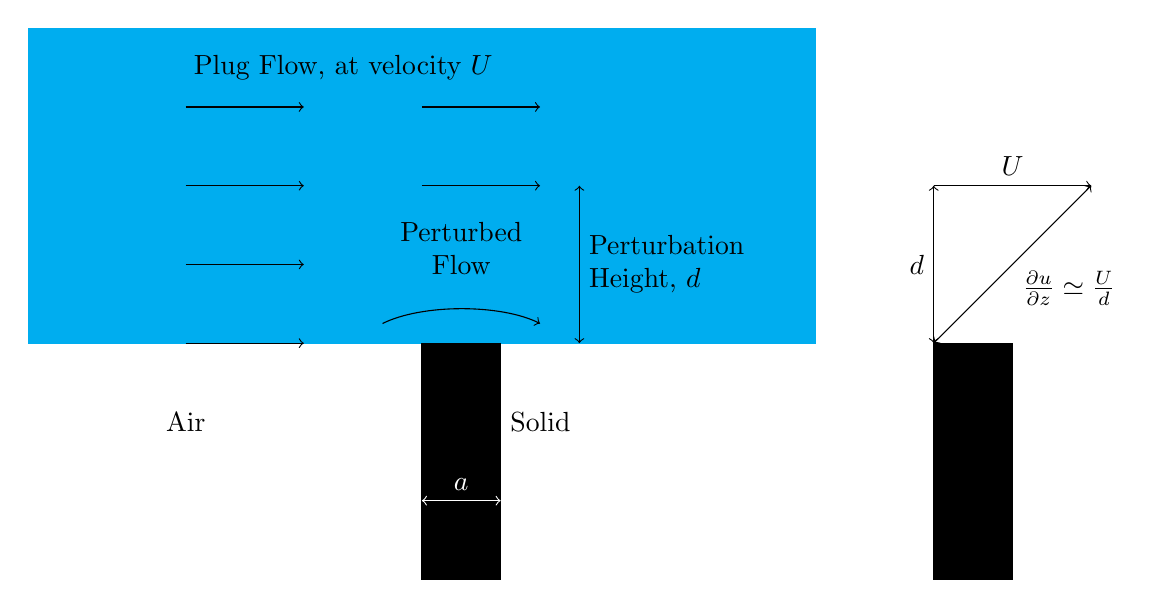
\begin{tikzpicture}

\filldraw[color=cyan] (-5,4) rectangle (5,0);
\filldraw (0,0) rectangle (1,-3);
\node at (-3,-1) {Air};
\node at (1,-1) [right] {Solid};

\draw [color=white, <->] (0,-2) -- node[above] {$a$} (1,-2);

\node at (-1,3.5) {Plug Flow, at velocity $U$};

\foreach \z in {0,1,2,3}
   \draw [->] (-3, \z) -- (-1.5, \z);
   
\node at (0.5,1.2) [align=center] {Perturbed\\Flow};
\draw [->] (-0.5,0.25) .. controls (0,0.5) and (1,0.5) .. (1.5, 0.25);
\foreach \z in {2,3}
   \draw [->] (0, \z) -- (1.5, \z);

\draw [<->] (2,0) -- node[right,align=left]{Perturbation\\Height, $d$} (2,2);


\filldraw (6.5,0) rectangle +(1,-3);
\draw [<->](6.5,0) -- node[left] {$d$} +(0,2);
\draw [->](6.5,2) -- node[above] {$U$} +(2,0);
\draw [<->](6.5,0) --  +(2,2);
\node at (7.5,0.7) [right] {$\frac{\partial u}{\partial z} \simeq \frac{U}{d}$};

\end{tikzpicture}

\vspace{1em}
The diagram shows flow over a surface comprising mostly fresh air.  The fluid is supported by surface tension on the tops of some widely-spaced nanopillars.

The bottom interface of the fluid is modelled as a flat plane with varying local boundary conditions:  Over the air, there is perfect slip;  Over the solid nanopillar, there is zero slip.  The nanopillars occupy some fraction \phisol  of the interface area.

Recall the fundamental physics of the Navier-Stokes equations: an element of fluid accelerates due to the net effect of pressure and viscous forces on it.  Stokes flow assumes acceleration is negligible, so that pressure and viscous forces cancel out: pressure = viscous drag.  Consider an infinitesimally small cube moving with a lamina of fluid. It experiences a viscous pull due to the fact that the lamina above it is moving at a slightly higher (or lower) speed.  Likewise, it experiences a viscous drag because the lamina below it is moving slightly slower.  The net effect of the viscous forces will be equal and opposite to the pressure drop along the cube.

Now consider an infinitesimal cube moving in the streamline at the boundary.  It experiences the same pressure drop and viscous pull from the faster layer above it, but drag force from the material below it is now a generalized \emph{friction} force - not necessarily viscous.

We'll now think in terms of force per unit area, the \emph{stress} $\sigma$. The viscous stress is a function of fluid viscosity $\eta$ and local shear rate $\dot{\gamma}(x)$.  The friction stress depends on local velocity $u$ and local friction coefficient $k$.
\[ \sigma_{\mathrm{viscous}} = \eta \dot{\gamma}(x), \;\;\;
\sigma_{\mathrm{friction}} = k(x) u(x) \]

Now, if there is \emph{no pressure gradient}, then the viscous force and friction force are opposite and equal.  But before demanding that there be no pressure gradient, we'll think about averaging.

We can \emph{average} the stresses at the boundary over some larger area of the boundary lamina.
\[ \langle \sigma_{\mathrm{viscous}} \rangle = \langle \eta \dot{\gamma}(x) \rangle = \eta \langle \dot{\gamma} \rangle, \;\;\;
\langle \sigma_{\mathrm{friction}} \rangle = \langle k(x) u(x) \rangle
 = k_{\mathrm{eff}} \langle u \rangle != \langle k \rangle \langle u \rangle \]

Cunningly, for a suitably chosen area, there may be no net pressure drop over it. 
Then the average stresses balance:
\[ \langle \sigma \rangle = \eta \langle \dot{\gamma} \rangle = 
 k_{\mathrm{eff}} \langle u \rangle \]

\textbf{Back to the problem.}
We choose the area of averaging to be the period of the inter-nanopillar spacing on the superhydrophobic surface.
The flow over a superhydrophobic surface is mostly over fresh air.  Over the air, perfect slip is assumed, that is, there is no shear in the fluid at the boundary.  The solution for Couette-type driven flow over a shear-free surface is \textbf{plug flow}.  Since the surface is \emph{mostly} shear-free, the flow profile will be close to plug flow. It has some characteristic velocity $U$.
As a corollary, there is \textbf{no stress} on the fluid from the air-water interface. Thus, the only stress is due to the nanopillars; the total stress over one period is simply the total stress on the nanopillar. Hence, the average stress over one period, is simply the average stress on the nanopillar, weighted by the fraction of the period that the pillar occupies.
\[ \langle \sigma \rangle = \phisol \eta \langle \dot{\gamma} \rangle_{\mathrm{pillar}} \]

The no-slip condition holds on the nanopillar. The presence of the nanopillar perturbs the plug flow profile, as fluid must slow down to zero velocity at the pillar surface.  At some height $d$ above the nanopillar, the fluid velocity is back to (within some arbitrary small fraction of) the plug velocity $U$.  Therefore, the velocity goes from 0 to $U$ in distance $d$, which is to say the velocity gradient is $U/d$.  The surface is flat, so simple shear obtains, and the shear rate is the velocity gradient.
\[ \langle \dot{\gamma} \rangle_{\mathrm{pillar}} = \frac{\partial u}{\partial z} \simeq \frac{U}{d} \]
Now, the height of perturbation $d$ scales as the width of the nanopillar, $a$, if all else is held constant. See Appendix D? So:
\[ \langle \dot{\gamma} \rangle_{\mathrm{pillar}} \simeq \frac{U}{a} \]

Therefore
\[ \langle \sigma \rangle \simeq \phisol \eta \frac{U}{a}  \]

Furthermore, $\langle \sigma \rangle = k_{\mathrm{eff}} \langle u \rangle$, so that
\[ k_{\mathrm{eff}} \langle u \rangle \simeq \phisol \eta \frac{U}{a}  \]
 
Another corollary of the fact that the flow is close to plug flow, is that the velocity on the boundary is mostly at the plug velocity $U$, with only a small region on and around the nanopillar with reduced velocity (including zero on the pillar).  Therefore, the \emph{average} boundary velocity over one period is strongly dominated by $U$:
\[ \langle u \rangle \simeq U \]
Thus:
\[ k_{\mathrm{eff}} U \simeq \phisol \eta \frac{U}{a}  \]

Cancel $U$ from both sides
\[ k_{\mathrm{eff}} \simeq \phisol \eta \frac{1}{a}  \]
Rearrange:
\[ \frac{a}{\phisol} \simeq \frac{\eta}{k_{\mathrm{eff}}} \]

Recall that for averaged velocities and shear rates, $\beff = \eta / k_{\mathrm{eff}}$. So finally
\[ \beff \simeq \frac{a}{\phisol} \]

\textbf{Effective Slip; Comparison with Tretheway and Meinhart}

At each point on the boundary, the Navier slip condition holds.
\[ u = b(x) \dot{\gamma}(x) \]
Averaging over one period:
\[ \langle u \rangle = \langle b \dot{\gamma} \rangle \]
Christophe defines
\[ \langle u \rangle = \beff \langle \dot{\gamma} \rangle  \]

Leibniz's Integration Rule states that if $f(x,z)$ and $\partial_z f(x,z)$ are both \emph{continuous} on a region $[x_0,x_1] \times [y_0,y_1]$ , then
\[ \frac{d}{dz} \int_{x_0}^{x_1} f(x,z) \;dx = 
\int_{x_0}^{x_1} \frac{\partial}{\partial z} f(x,z) \;dx  \]

Therefore, it is true that for a smooth velocity function
\[ \langle \dot{\gamma} \rangle = \langle \partial_z u \rangle =
\partial_z \langle u \rangle \]

Hence Christophe is saying that for a smooth velocity field
\[ \langle u \rangle = \beff \partial_z \langle u \rangle \]

Sadly, this does not imply $\beff = \langle b \rangle $.

\vspace*{1em}
Contrast this with Tretheway and Meinhart.  I \emph{believe} they defined 
\[ \langle u \rangle = \beff \partial_z \langle u \rangle \] where the averages are over a binary surface.  By Leibniz, $\partial_z \langle u \rangle =  
\langle \partial_z u \rangle$.  Crucially, the shear rate over a (pure) no-slip surface is the same as the shear rate over a rarefied gas layer.  So $\partial_z u$ is \emph{constant.} Hence
\[ \langle u \rangle = \beff \dot{\gamma}_{\mathrm{const}} \]
Therefore, using the construction
\[ \langle u \rangle = \langle b(x) \dot{\gamma}_{\mathrm{const}} \rangle 
= \langle b(x) \rangle \dot{\gamma}_{\mathrm{const}} \]
That is to say:
\[ \beff = \langle b \rangle \]
This results from the naive definition of `cumulative velocity' -- a superposition of solutions of the pure no-slip and slip cases, and the concomitant identical shear rates.

Christophe makes no such absurd assumption.


\subsubsection*{Other Results}

Moving on.  Christophe compares to J. Phillip's exact result for the groove geometry.
\[ \beff = \frac{-L}{\pi} \log \left[ \cos \left( \frac{\pi}{2} (  1-\phisol) \right) \right] \]

In the limit of vanishing $\phisol$, $\cos(\pi/2 ( 1- \phisol)) $ is very close to $\pi/2$, where the function is very close to linear, with slope = -1.  Therefore, 
$\cos(\pi/2 ( 1- \phisol)) \sim \phisol $, so ``$\beff$ [depends] only logarithmically through $\beff \sim -L \log \phisol $.  For this groove geometry, the solid fraction simply reads $\phisol = a/L$ so that the scaling law approach now becomes
\[ \beff \sim L,\;\;\;{\phisol \rightarrow 0}." \]

Considering now a surface consisting of a nanoforest of nanopillars, the solid fraction now reads $\phisol = (a/L)^2$ so that we have
\[ \beff \sim \frac{a}{ \sqrt{\phisol} } \]

Finally, Christophe relaxes the no-slip condition on the solid part, allowing an intrinsic slip length $b_s$. Then, the shear rate over the solid regions is reduced: 
$\langle \dot{\gamma}_w \rangle_s \sim U/(a + b_s) $ ``The averaged shear stress over the total surface now reads $ \langle \sigma_w \rangle = \phisol \eta U/(a + b_s) $.  One gets accordingly a modified scaling law for the effective slip length,
\[ \beff \sim \frac{a+b_s}{\phisol}. \]

\textbf{Limit of vanishing gas areas: $\phisol \rightarrow 1$}

This limit has much less practical value. But for completeness, the flow will be essentially Couette flow except over the gas-filled groove, which has characteristic length scale $l$. Then
\[ \beff \sim l(1-\phisol) \]

\textbf{Towards a general description for the slip length.}

Moving on from `ideal' surfaces, the air-water interface is not assumed to be shear free, but instead considered to have a finite slip length $b_g$. First consider the limit $b_g \rightarrow 0$. Then the velocity profile will be approximately $u(x,y,z) = \dot{\gamma} [z + b(x,y)]$.  ``The averaged velocity profile thus reads 
$ \langle u \rangle (z) = \dot{\gamma}(z + \langle b \rangle ) $. Using the definition of the effective slip length, this velocity profile is expected to identify with $\langle u \rangle (z) = \dot{\gamma}(z + \beff ) $. This yields the following expression for the effective slip length in this limit:
\[ \beff = (1 - \phisol) b_g." \]

``For large $b_g$, no such simple prediction could be obtained."  Define $b_{\mathrm{ideal}}$ as the effective slip length obtained from assuming a shear-free air-water interface ($b_g \rightarrow \infty$).  Then a heuristic formula interpolating between the limits $ b_g \rightarrow 0$ and $b_g \rightarrow \infty$ is:
\[ \frac{1}{\beff} = \frac{1}{(1-\phisol) b_g} + \frac{1}{b_{\mathrm{ideal}}}. \]

\textbf{Effect of Curvature}

If the gas has a meniscus bulging \emph{into} the liquid by distance $\delta$, this causes a friction which can be described by a slip length $b_g \sim l^2 / \delta$, where $l$ is the length scale of the gas eg. bubble radius.  This result is from Einzel, Panzer and Liu, but they offer a simple scaling argument derivation also.

They consider the case of grooves parallel to flow, with period $L$.
They put this into the interpolation formula.  In the interesting limit of small solid fraction, this is:
\[ \frac{1}{\beff} = \frac{\delta}{ L^2 } + \frac{1}{b_{\mathrm{ideal}}} \]

\textbf{Discussion, Putting it together.}
They look at at practical superhydrophic surface with period $L$. They consider the `macroscopic observable ... effective contact angle $\theta_{\mathrm{eff}}$' Then for contact angles close to $180^{\circ}$, the effective slip length diverges as
\[ \beff \propto \frac{L}{180 - \theta_{\mathrm{eff}}} \]


\subsubsection*{Hendy and Lund 2007}
\textbf{Flat Surface \\ Periodic Slip Pattern \\ Intrinsic Slip Larger than Period; otherwise arbitrary \\ Stokes Flow}


In which Shaun uses his Fourier series approach to prove that
\[ \beff = \left< \frac{1}{b(x,y)} \right>^{-1} \]
for a \emph{flat} surface with a periodic variation in slip length of period $L$, where the intrinsic slip length $b(x,y) \gg L$ everywhere.


\subsubsection*{Ng and Wang 2009}
\textbf{Partial Slip/ Infinite Slip \\ Flow Parallel and Transverse to Grating \\ Non Flat! Liquid Penetrates into Gas-Filled Grooves \\ Stokes Flow}

These guys consider flow (in both transverse and parallel orientations) over a grating: solid slats with a square cross section, separated by liquid-gas interface located distance $d$ below the tops of the slats.  There is a local slip length $b \geq 0$ on the solid, and the liquid-gas interface has perfect slip.

\vspace*{1em}
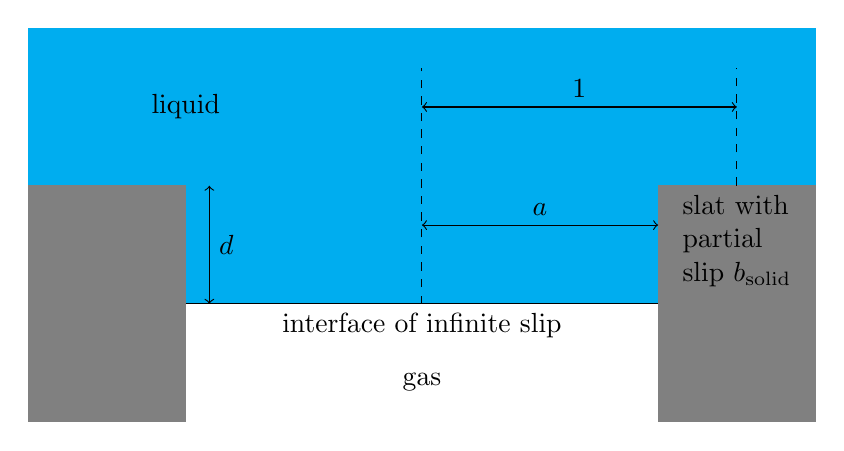
\begin{tikzpicture}
\filldraw[color=cyan] (-5,-1.5) rectangle (5,2);

\filldraw[color=gray] (-3,0) rectangle +(-2,-3);
\filldraw[color=gray] (3,0) rectangle +(2,-3);

\draw (-3,-1.5) -- node[below]{interface of infinite slip} +(6,0);
\node at (-3,1) {liquid};
\node at (0,-2.5) {gas};
\node at (4,0)[below, align=left] {slat with\\partial\\slip $b_{\mathrm{solid}}$};

\draw[<->] (-2.7,0) -- node[right]{$d$} +(0,-1.5);

\draw[dashed] (0,-1.5) -- +(0,3);
\draw[dashed] (4,0) -- +(0,1.5);

\draw[<->] (0,-0.5) -- node[above]{$a$} +(3,0);
\draw[<->] (0,1) -- node[above]{1} +(4,0);

\end{tikzpicture}

They derive semi-analytic solutions for flow both transverse and parallel to the slats.  Eigenfunction expansions are solved numerically to derive effective slip lengths.  They compare their numerical results with the continuum modeling results of Cottin-Bizonne \emph{et al.} in the 2004 Eur. Phys. Journal; agreement is essentially perfect.

They note that Cottin-Bizonne proposed a phenomenological model for effective slip of slats parallel to flow:
\[ \beff = \frac{b_{\mathrm{solid}}}{1-a} \;\;\; \text{for } d = 0. \]
which works very well for large $b_{\mathrm{solid}}$. Ng and Wang have discovered that this can be improved to work for the full range of $b_{\mathrm{solid}}$ by simply adding John Philip's exact result for $b_{\mathrm{solid}} = 0$. So that:

\[ \beff = \frac{2}{\pi} \ln \left[ \sec \left( \frac{\pi a}{2} \right) \right]
 + \frac{b_{\mathrm{solid}}}{1-a} \;\;\; \text{for } d = 0. \]
 
 Or in notation consistent with the rest the review: $L$ is period and $\phi$ is fraction of surface with perfect slip. 
 \[ \beff = \frac{L}{\pi} \ln \left[ \sec \left( \frac{\pi}{2} \phi \right) \right]
 + \frac{b_{\mathrm{solid}}}{1-\phi} \;\;\; \text{for } d = 0. \]
 
Similarly for flow transverse to the slats:
\[ \beff = \frac{1}{2} \frac{L}{\pi} \ln \left[ \sec \left( \frac{\pi}{2} \phi \right) \right]
 + \frac{b_{\mathrm{solid}}}{1-\phi} \;\;\; \text{for } d = 0. \]

Ng and Wang test these extended formulae numerically, and find that they have a maximum error of 3\% -- 6\%, compared with Cottin-Bizonne's original formula which can have a maximum error of more that 50\% for small $b_{\mathrm{solid}}$.

\vspace*{1em}
Ng and Wang then spend several pages in qualitative discussion about the degree to which the fluid penetrates down between the slats.  The only thing worthy of making it into their summary is this: a very small increase in $d$ is enough to drastically reduce the effective slip length, particularly for the transverse flow case.


\subsubsection*{Davis and Lauga PoF 2009a}

\textbf{No-slip/Perfect-slip}\\
\textbf{Not flat!  Circular bubbles}\\
\textbf{Analytical result for dilute limit - sparse bubble coverage}
\textbf{2-dimensional Stokes flow}\\

Davis and Lauga consider 2-dimensional Stokes flow over a flat surface \textbf{sparsely} covered with circular holes.  Air in the holes forms spherical bubbles.  The greater the gas pressure in the bubble, the more the bubble protrudes into the liquid.  This is quantified by angle of the bubble wall to the horizontal plane.  No slip is assumed on the flat solid, and perfect slip on the bubbles.

\vspace*{1em}

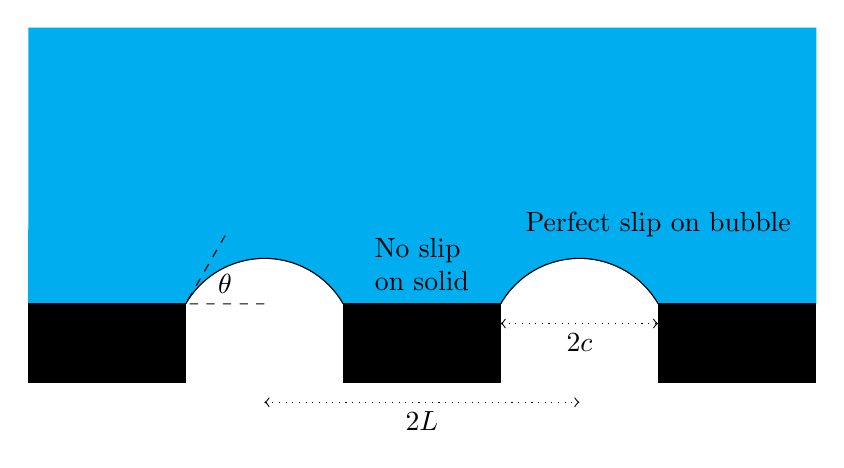
\begin{tikzpicture}
\filldraw[color=cyan](0,0) -- ++(2,0) arc (150:30:1.155cm) 
-- ++(2,0) arc (150:30:1.155cm) -- ++(2,0) 
-- ++(0,3.5) -- ++(-10,0);

\filldraw[color=black] (0,0) rectangle +(2,-1);
\draw (2,0) arc (150:30:1.155cm);
\filldraw[color=black] (4,0) rectangle +(2,-1);
\draw (6,0) arc (150:30:1.155cm);
\filldraw[color=black] (8,0) rectangle +(2,-1);

\draw[dashed] (3,0) -- (2,0) -- (2.5, 0.866);
\node at (2.5,0.25) {$\theta$};

\draw[<->,dotted] (6,-0.25) -- node[below]{$2c$}  +(2,0);
\draw[<->,dotted] (3,-1.25) -- node[below]{$2L$} +(4,0);

\node at (5,0.5)[align=left] {No slip\\ on solid};
\node at (8,1) {Perfect slip on bubble};

\end{tikzpicture}
\vspace*{1em}

By using stream functions and conformal mapping (remember it is 2-D flow), they get an analytic result for the effective slip length:

\[
\beff = c \pi \left( \frac{c}{L} \right) \int_0^{\infty}
\frac{s}{\sinh 2s(\pi - \theta) + s \sin 2 \theta}
\left[ \cos 2 \theta +
\frac{s \sin 2 \theta \cosh s \pi + \sinh s(\pi - 2 \theta)}{\sinh s \pi}
\right] \; ds
\]

valid in the dilute limit -- sparse coverage of bubbles.

They evaluate for various values of $\theta$, nondimensionalized by bubble-hole radius $c$.  They find good agreement with the numerical results of Steinberger \emph{et al} and Hyvaluoma and Harting.

``The main features of the full numerical results are seen to be reproduced by our analytical model.  There exists a critical protrusion angle $\theta_c$ above which the effect of the wall-attached bubbles displays a transition from reduced ($\theta < \theta_c$) to enhanced friction ($\theta > \theta_c$).  Our model predicts $\theta_c \approx 65^{\circ}$, in good agreement with the results of [Steinberger \emph{et al}] ($\theta_c \approx 62^{\circ}$) and [Hyvaluoma and Harting] ($\theta_c \approx 69^{\circ}$)."


\subsubsection*{Davis and Lauga 2009b}
\textbf{No-slip/Perfect-slip \\ Flat \\ 2-D mesh of solid strips \\ Stokes flow
\\ Analytic solution in limit of small strip width.}

They consider Stokes flow over a mesh of thin wires or strips, with large square air gaps in between.  The surface is considered flat, and slip length is zero on the strips, and infinite on the air-water interfaces.  The period of the square-periodic mesh is $L$, and the width of the strips is $\epsilon L$.
\vspace*{1em} 

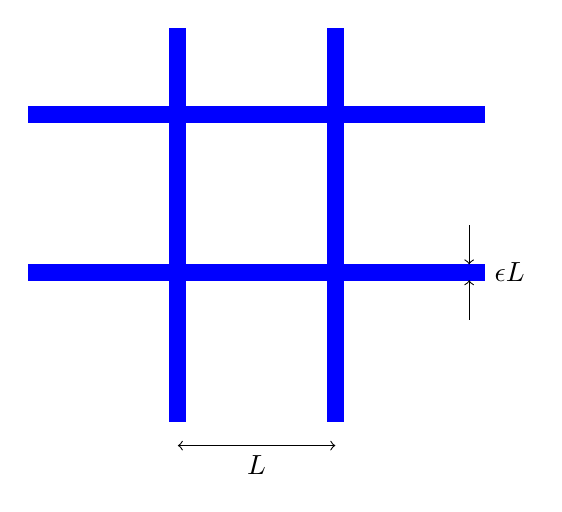
\begin{tikzpicture}

\filldraw[color=blue] (0,0) rectangle +(0.2,5);
\filldraw[color=blue] (2,0) rectangle +(0.2,5);
\draw[<->] (0.1,-0.3) -- node[below]{$L$} +(2,0);

\filldraw[color=blue] (-1.8,2) rectangle +(5.8,-0.2);
\filldraw[color=blue] (-1.8,4) rectangle +(5.8,-0.2);
\draw[<-] (3.8,2) -- +(0,0.5);
\draw[<-] (3.8,1.8) -- +(0,-0.5);
\node at (4,1.9)[right] {$\epsilon L$};

\end{tikzpicture}

\vspace*{1em}
Davis and Lauga use a method of superposition of singularities, and end up with an infinite system of linear equations.  The effective slip length is:

\[ \beff = \frac{L}{\pi (A_0 + B_0)} \]
where $A_0$ and $B_0$ are the zeroth-order coefficients of the system of linear equations.

They solve numerically for $A_0$ and $B_0$ by truncating the infinite system at $N$ equations.  Truncating at $N=1000$ compared to $N=100$ changed the computed effective slip length by less than 0.01\%. After computing $\beff$ for various values of $\epsilon$, they derive a least-squares fit formula:
\[ \frac{\beff}{L} = -0.107 \ln \epsilon - 0.069 \]
Or, if one thinks in terms of solid fraction rather than strip width:
\[ \frac{\beff}{L} = -0.107 \ln \phisol + 0.003 \] 

Finally, they offer `simple estimates' -- solutions from truncating the infinite series at $N=1$ and $N=2$ terms.  For $N=1$:

\[ \frac{\beff}{L} = \frac{1}{3 \pi} \ln \left( \frac{2}{\pi \epsilon} \right) \]

Let $\ln \left( \frac{2}{\pi \epsilon} \right) = \beta$.  Then for $N=2$:

\[ \frac{\beff}{L} = \frac{1}{3 \pi}\beta - \frac{\beta + \frac{1}{2}}
{6\pi \left[ \beta^2 + \frac{1}{4}\beta - \frac{1}{2} + \frac{9}{4 \sqrt{2}} 
\left( \beta + \frac{1}{2} \right) 
\right] }\]

These simple estimates overestimate $\beff$ by up to 10\%, but converge on the correct result as $\epsilon \rightarrow 0$.



\subsubsection*{Ng and Wang 2010}
\textbf{Flat\\ Perfect slip\\ No slip and partial slip\\ 2-D patterns of holes or posts\\ Fit Ybert's scaling laws to numerical data; present fitted parameters. }

These guys take the scaling laws suggested by Ybert in 2007, and refine them with parameters calculated by fitting to numerical data.  They solve Stokes flow over a flat surface by the method of eigen function expansions, then solve the system of equations numerically.

For superhydrophobic surfaces, i.e. flow over posts, the solid fraction is small.  Ybert proposed:
\[ \beff \sim \phisol^{-1/2} \;\;\; \text{for} \;\;\; \phisol \rightarrow 0 \]

Ng and Wang fit parameters to their numerical data, getting:
\[ \beff = 0.34 \phisol^{-1/2} - 0.468 \;\;\; \text{for circular posts,} \]
\[ \beff = 0.33 \phisol^{-1/2} - 0.461 \;\;\; \text{for square posts,} \]

For flow over holes or nanobubbles, there is a contiguous solid area of low or no slip, so effective slip is reduced compared to the superhydrophobic geometry with the same solid fraction.  In 2007, Ybert proposed
\[ \beff \sim - \ln \phisol \;\;\; \text{for} \;\;\; \phisol \rightarrow 0 \]

Ng and Wang find parameters:
\[ \beff = -0.115 \ln \phisol - 0.014 \;\;\; \text{for square holes,} \]
\[ \beff = -0.134 \ln \phisol - 0.023 \;\;\; \text{for circular holes,} \]


Ng and Wang then move from the no-slip/perfect-slip regime to one where slip is allowed on the solid parts.  They present a table of fitted parameters for square and circular holes and posts for three different intrinsic slip lengths.  Have a look if you care.

Lastly, they look at changing the aspect ratio i.e. ellipses and rectangles rather than symmetric circles and squares.  They present a bunch of fitted coefficients.



\subsubsection*{Davis and Lauga 2010}
\textbf{Flat\\ Superhydrophobic: circular posts in rectangular array
\\ No-slip/Perfect-slip\\ Stokes flow}

Davis and Lauga again take Ybert 2007 as a point of departure. They consider Stokes flow over a superhydrophobic surface comprising a rectangular array of circular posts, each of radius $a$.
\vspace*{1em}

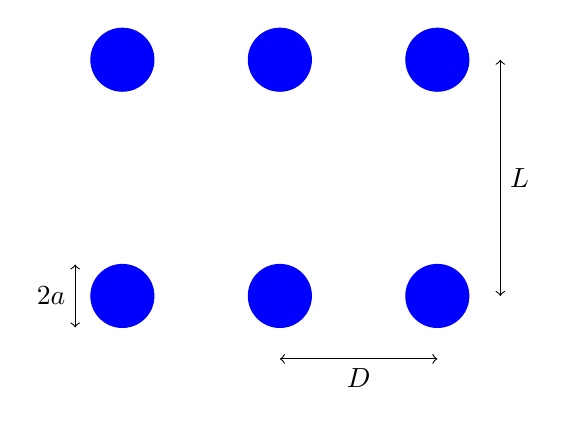
\begin{tikzpicture}

\filldraw[color=blue] (0,0) circle (4mm);
\filldraw[color=blue] (2,0) circle (4mm);
\filldraw[color=blue] (4,0) circle (4mm);
\filldraw[color=blue] (0,3) circle (4mm);
\filldraw[color=blue] (2,3) circle (4mm);
\filldraw[color=blue] (4,3) circle (4mm);

\draw[<->] (-0.6,-0.4) -- node[left]{$2a$} +(0,0.8);
\draw[<->] (2,-0.8) -- node[below]{$D$} +(2,0);
\draw[<->] (4.8,0) -- node[right]{$L$} +(0,3);

\end{tikzpicture}
\vspace*{1em}

They begin by noting that Ybert in 2007 proposed that in the limit of low $\phisol$
\[ \frac{\beff}{L} \sim \frac{A}{\sqrt{\phisol}} - B \]

They attack the problem with Fourier transform techniques, and end up with an infinite system of linear equations for coefficients $c_n$.  They make an `asymptotic estimate' of the coefficients, and get 
\[ \frac{\beff}{\sqrt{DL}} \sim \frac{3}{16} \sqrt{\frac{\pi}{\phisol}} \]

For the square case, $D=L$ and
\[ \frac{\beff}{L} \sim \frac{3}{16} \sqrt{\frac{\pi}{\phisol}} \]

Adding the next-order correction term (simplest for the square array) gives:
\[ \frac{\beff}{L} \sim \frac{3}{16} \sqrt{\frac{\pi}{\phisol}}
- \frac{3}{2 \pi} \ln (1 + \sqrt{2}) \]
in the limit of low $\phisol$.

They compare their analytical asymptotic estimate with previous numerical work: ``The quantitative agreement between our model and previous numerical work is remarkable... we find that the error between our simple model, and the numerics of Ng and Wang (2010) is about 1.8\%, while the error between our model and the computations of Ybert \emph{et al.} (2007) is about 3.9\%."

\end{document}